\let\lesson\undefined
\newcommand{\lesson}{\phantomlesson{Bài 3: Nội năng. Định luật 1 nhiệt động lực học}}
\chapter[Nội năng]{Nội năng}
\section{Lý thuyết}
\subsection{Nội năng}
\subsubsection{Khái niệm nội năng}
Nội năng của một vật là tổng động năng và thế năng tương tác của các phân tử cấu tạo nên vật. Nội năng của vật phụ thuộc vào nhiệt độ $T$ và thể tích $V$ của vật:
$$U=f\left(T, V\right).$$
Đơn vị của nội năng trong hệ SI là joule $\left(\si{\joule}\right)$.
\subsubsection{Mối liên hệ giữa nội năng và năng lượng của các phân tử cấu tạo nên vật}
Khi năng lượng của các phân tử cấu tạo nên vật tăng thì nội năng của vật tăng và ngược lại.
\subsection{Các cách làm thay đổi nội năng}
\subsubsection{Thực hiện công}
Quá trình thực hiện công làm cho nội năng của hệ thay đổi, hệ nhận công thì nội năng của hệ tăng, hệ thực hiện công cho vật khác thì nội năng giảm.\\
\textbf{\textit{Ví dụ 1:}} Dùng tay ấn mạnh và nhanh piston của một cylanh chứa khí, thể tích khí trong cylanh giảm xuống (thế năng tương tác giữa các phân tử khí tăng), đồng thời khí nóng lên (động năng chuyển động nhiệt của các phân tử khí tăng). Do đó, nội năng của khí tăng.\\
\textbf{\textit{Ví dụ 2:}} Chà xát hai thanh gỗ với nhau, bề mặt tiếp xúc của hai thanh gỗ nóng dần lên. Nội năng của thanh gỗ tăng.
\begin{center}
	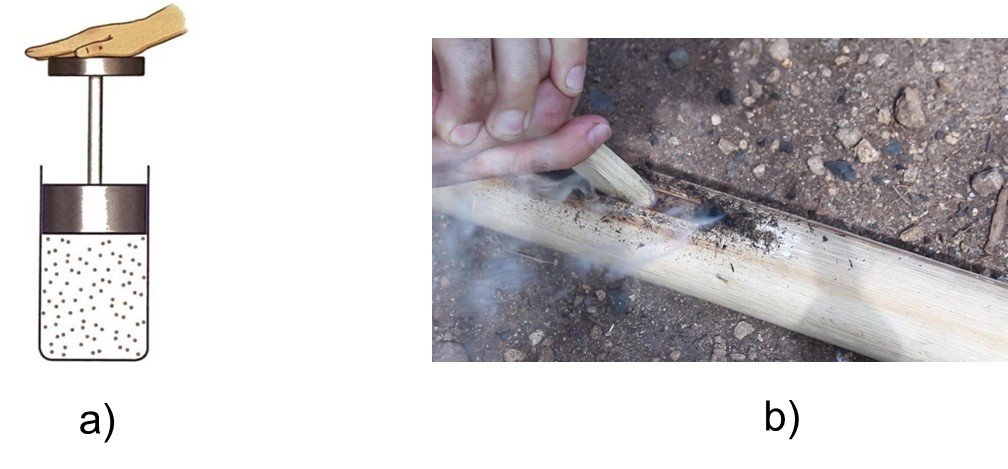
\includegraphics[width=0.45\linewidth	]{../figs/VN12-Y24-PH-SYL-003-1}
	\captionof{figure}{a) Nén khối khí trong cylanh; b) Chà xát hai thanh gỗ với nhau.}
\end{center}
\subsubsection{Truyền nhiệt}
Quá trình làm thay đổi nội năng của vật bằng cách cho nó tiếp xúc với vật khác khi có sự chênh lệch nhiệt độ giữa chúng gọi là sự truyền nhiệt.\\
\textbf{\textit{Ví dụ:}} Miếng sắt sau khi tôi luyện được thả vào chậu nước để làm nguội đi. Khi đó, nước nhận nhiệt lượng từ miếng sắt nên nội năng tăng (nhiệt độ tăng) và miếng sắt truyền nhiệt lượng cho nước nên nội năng giảm (nhiệt độ giảm).
\begin{center}
	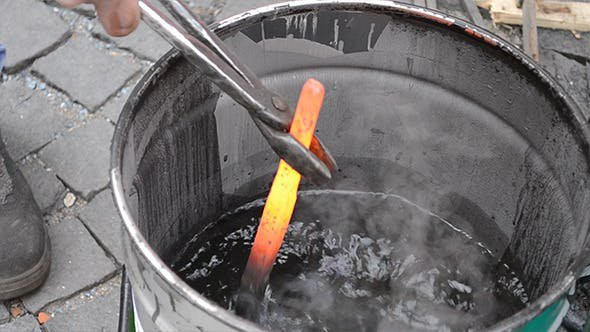
\includegraphics[width=0.3\linewidth]{../figs/VN12-Y24-PH-SYL-003-2}
	\captionof{figure}{Miếng sắt nung được thả vào chậu nước.}
\end{center}
\subsection{Định luật I nhiệt động lực học}
Độ biến thiên nội năng của hệ bằng tổng công và nhiệt lượng mà hệ nhận được:
\begin{equation}
	\Delta U= A+Q
\end{equation}
Trong đó:
\begin{itemize}
	\item $\Delta U$: độ biến thiên nội năng của hệ, đơn vị trong hệ SI là joule $\left(\si{\joule}\right)$;
	\item $A$: công mà hệ nhận/thực hiện, đơn vị trong hệ SI là joule $\left(\si{\joule}\right)$;
	\begin{itemize}[label=+]
		\item $A>0$: hệ nhận công;
		\item $A<0$: hệ thực hiện công.
	\end{itemize}
	\item $Q$: nhiệt lượng hệ trao đổi với bên ngoài, đơn vị trong hệ SI là joule $\left(\si{\joule}\right)$;
	\begin{itemize}[label=+]
		\item $Q>0$: hệ nhận nhiệt lượng;
		\item $Q<0$: hệ truyền nhiệt lượng.
	\end{itemize}
\end{itemize}
\begin{center}
	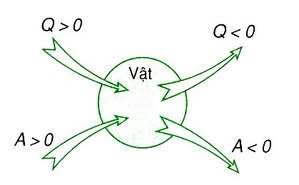
\includegraphics[width=0.35\linewidth]{../figs/VN12-Y24-PH-SYL-003-3}
	\captionof{figure}{Quy ước về dấu của $Q$ và $A$.}
\end{center}
\section{Mục tiêu bài học - Ví dụ minh hoạ}
\begin{dang}{Trình bày được các cách làm thay đổi nội năng
	}
	\viduii{2}
	{Dựa vào mô hình động học phân tử, hãy giải thích hiện tượng quả bóng bàn bị móp (nhưng chưa bị thủng) khi thả vào cốc nước nóng sẽ phồng trở lại.
		\begin{center}
			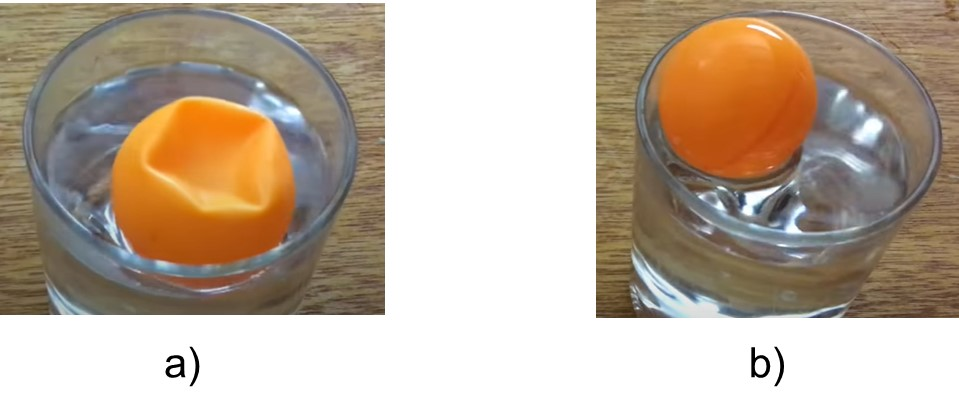
\includegraphics[width=0.45\linewidth]{{../figs/VN12-Y24-PH-SYL-003-4}}
			\captionof{figure}{a) Quả bóng bàn ban đầu bị móp; b) Quả bóng sau khi được ngâm vào cốc nước nóng.}
		\end{center}
	
}
{\hide{
	Khi thả quả bóng bi móp vào nước nóng, nhiệt độ khí trong quả bóng tăng làm các phân tử khí chuyển động nhiệt nhanh hơn nên va chạm với thành bóng nhiều hơn và mạnh hơn. Khi đó, áp suất khí trong quả bóng tăng lên và tạo ra lực đẩy đủ lớn làm vỏ cao su của quả bóng phồng trở lại.}
}

\viduii{2}
{Vì sao pha nước chanh bằng nước ấm thì đường sẽ tan nhanh hơn khi pha bằng nước lạnh? Em còn cách làm nào khác để đường tan nhanh hơn không? Hãy đưa ra lời giải thích cho cách làm của em.
}
{\hide{Khi nhiệt độ càng cao thì động năng chuyển động nhiệt của các phân tử nước và phân tử đường càng lớn. Do đó, các phân tử đường dễ dàng hoà tan vào trong nước.\\
Để đường tan nhanh vào nước ta có thể khuấy mạnh vào nước. Khi đó, hệ nước và đường nhận công nên động năng chuyển động của các phân tử đường và nước tăng. Các phân tử đường dễ hoà tan vào nước.}
}

\end{dang}
\begin{dang}{Vận dụng định luật I nhiệt động lực học}
	\viduii{2}
	{Giả sử cung cấp cho hệ nhiệt động một công là $\SI{200}{\joule}$ nhưng nhiệt lượng mà hệ bị thất thoát ra ngoài môi trường là $\SI{120}{\joule}$. Hỏi nội năng của hệ tăng hay giảm bao nhiêu?
	
}
{\hide{Hệ nhận công nên $A>0\Rightarrow A=\SI{200}{\joule}$.\\
	Hệ toả nhiệt ra ngoài môi trường nên $Q<0\Rightarrow Q=\SI{-120}{\joule}$.\\
Độ biến thiên nội năng của hệ:
$$\Delta U= Q+A=\SI{80}{\joule}.$$
Vậy nội năng của hệ tăng $\SI{80}{\joule}.$}
}

\viduii{3}
{Cung cấp nhiệt lượng $\SI{1.5}{\joule}$ cho một khối khí trong một cylanh đặt nằm ngang. Chất khí nở ra, đẩy piston đi một đoạn $\SI{5}{\centi\meter}$. Biết lực ma sát giữa piston và cylanh có độ lớn là $\SI{20}{\newton}$, coi piston chuyển động thẳng đều. Tính
	\begin{enumerate}[label=\alph*)]
		\item Công của khối khí thực hiện.
		\item Độ biến thiên nội năng của khối khí.
	\end{enumerate}

}
{\hide{
\begin{enumerate}[label=\alph*)]
	\item Do piston chuyển động thẳng đều nên lực đẩy $\vec{F}$ của khối khí tác dụng lên lên piston cân bằng với lực ma sát giữa piston và cylanh.\\
	Độ lớn công của khối khí thực hiện là:
	$$A'=F\cdot d=F_\text{ms}\cdot d=\left(\SI{20}{\newton}\right)\cdot\left(\SI{0.05}{\meter}\right)=\SI{1}{\joule}.$$
	\item Vì khối khí thực hiện công nên $A<0$: $A=-A'=\SI{-1}{\joule}$.\\
	Khối khí nhận nhiệt nên $Q>0\Rightarrow Q=\SI{1.5}{\joule}$.\\
	Độ biến thiên nội năng của khối khí:
	$$\Delta U=Q+A=\SI{1.5}{\joule}-\SI{1}{\joule}=\SI{0.5}{\joule}.$$
	Vậy nội năng của khối khí tăng $\SI{0.5}{\joule}$.
\end{enumerate}}
}

\viduii{3}
{Khi truyền nhiệt lượng $Q$ cho khối khí trong một cylanh hình trụ thì khí dãn nở đẩy piston làm thể tích của khối khí tăng thêm 7 lít. Biết áp suất của khối khí là $\SI{3E5}{\pascal}$ và không đổi trong quá trình khí dãn nở. Tính
	\begin{enumerate}[label=\alph*)]
		\item Công mà khối khí thực hiện.
		\item Nhiệt lượng cung cấp cho khối khí. Biết rằng trong quá trình này, nội năng của khối khí giảm $\SI{1100}{\joule}$.
	\end{enumerate}

}
{\hide{
	\begin{enumerate}[label=\alph*)]
		\item Độ lớn công khối khí thực hiện:
		$$A'=F\cdot d=p\cdot S\cdot d=p\cdot\Delta V=\left(\SI{3E5}{\pascal}\right)\cdot\left(\SI{7E-3}{\meter^3}\right)=\SI{2100}{\joule}.$$
		\item Vì khối khí thực hiện công nên $A<0$: $A=-A'=\SI{-2100}{\joule}$.\\
		Nội năng của khí giảm nên $\Delta U<0\Rightarrow \Delta U=\SI{-1100}{\joule}$.\\
		Áp dụng định luật I nhiệt động lực học, nhiệt lượng cần cung cấp cho khối khí:
		$$Q=\Delta U - A=\SI{-1100}{\joule}+\SI{2100}{\joule}=\SI{1000}{\joule}.$$
	\end{enumerate}
}
}
\end{dang}